\documentclass{article}

\usepackage{icml2025}
\usepackage{amsmath}
\usepackage{amssymb}
\usepackage{graphicx}
\usepackage{hyperref}
\usepackage{booktabs}

\icmltitlerunning{Learning Activation Functions via Correlation Objectives}

\begin{document}

\twocolumn[
\icmltitle{Learning Activation Functions via Correlation Objectives}

\begin{icmlauthorlist}
\icmlauthor{Anonymous}{anon}
\end{icmlauthorlist}

\icmlaffiliation{anon}{Anonymous Institution}

\icmlcorrespondingauthor{Anonymous}{anonymous@example.com}

\icmlkeywords{activation functions, deep learning, correlation learning, Swish, representation learning}

\vskip 0.3in
]

\begin{abstract}
Neural networks rely on activation functions chosen heuristically before training, such as ReLU, Swish, or GELU. While these choices are motivated by empirical performance and mathematical properties like non-saturating gradients, a principled derivation from first principles remains elusive. We present a theoretical framework for deriving optimal activation functions by optimizing correlation-based objectives. For Gaussian mixture inputs, we obtain closed-form solutions revealing that Swish-like activations ($f(x) \approx x \cdot \sigma(\beta x)$) emerge naturally as optimal for moderate class separation. We validate this theory empirically: deep networks trained on CIFAR-10 with learnable piecewise-linear activations converge to shapes closely matching our theoretical predictions. Our work provides a principled foundation for understanding and designing activation functions, connecting optimization objectives to emergent functional forms.
\end{abstract}

\section{Introduction}
\label{sec:intro}

Activation functions are fundamental building blocks of neural networks, introducing nonlinearity that enables learning of complex representations. Standard choices like ReLU~\citep{glorot2011relu,nair2010relu}, Swish~\citep{ramachandran2017swish}, and GELU~\citep{hendrycks2016gelu} are selected before training based on heuristics: non-saturating gradients, smoothness, computational efficiency, or biological plausibility. While these functions have proven effective empirically, their design remains largely ad-hoc.

A natural question arises: \textit{Can we derive optimal activation functions from task objectives and data statistics, rather than choosing them a priori?} This would provide both theoretical insight into why certain functional forms work well and a principled approach to designing new activations.

We address this question through a correlation-based optimization framework. For a unit receiving input $x$ with class label $y$, we define the \textit{class-wise correlation} $\rho_k = \text{Corr}(f(x), \mathbb{1}[y=k])$ and optimize an objective that encourages positive correlations while penalizing negative ones. This creates a natural competition between classes due to the zero-sum constraint $\sum_k \rho_k = 0$.

\textbf{Main contributions:}
\begin{itemize}
\item We derive closed-form optimal activation functions for Gaussian mixture inputs, revealing structure-from-statistics principles.
\item For moderate class separation, Swish-like activations ($f(x) = x \cdot \sigma(\beta x)$) emerge naturally—not by design, but as the optimal solution.
\item We validate theory empirically: VGG and ResNet trained on CIFAR-10 with learnable activations converge to shapes matching theoretical predictions.
\item We provide analytical understanding of why Swish works: correlation budget constraints combined with smooth gating produce this functional form.
\end{itemize}

\begin{figure}[t]
\centering
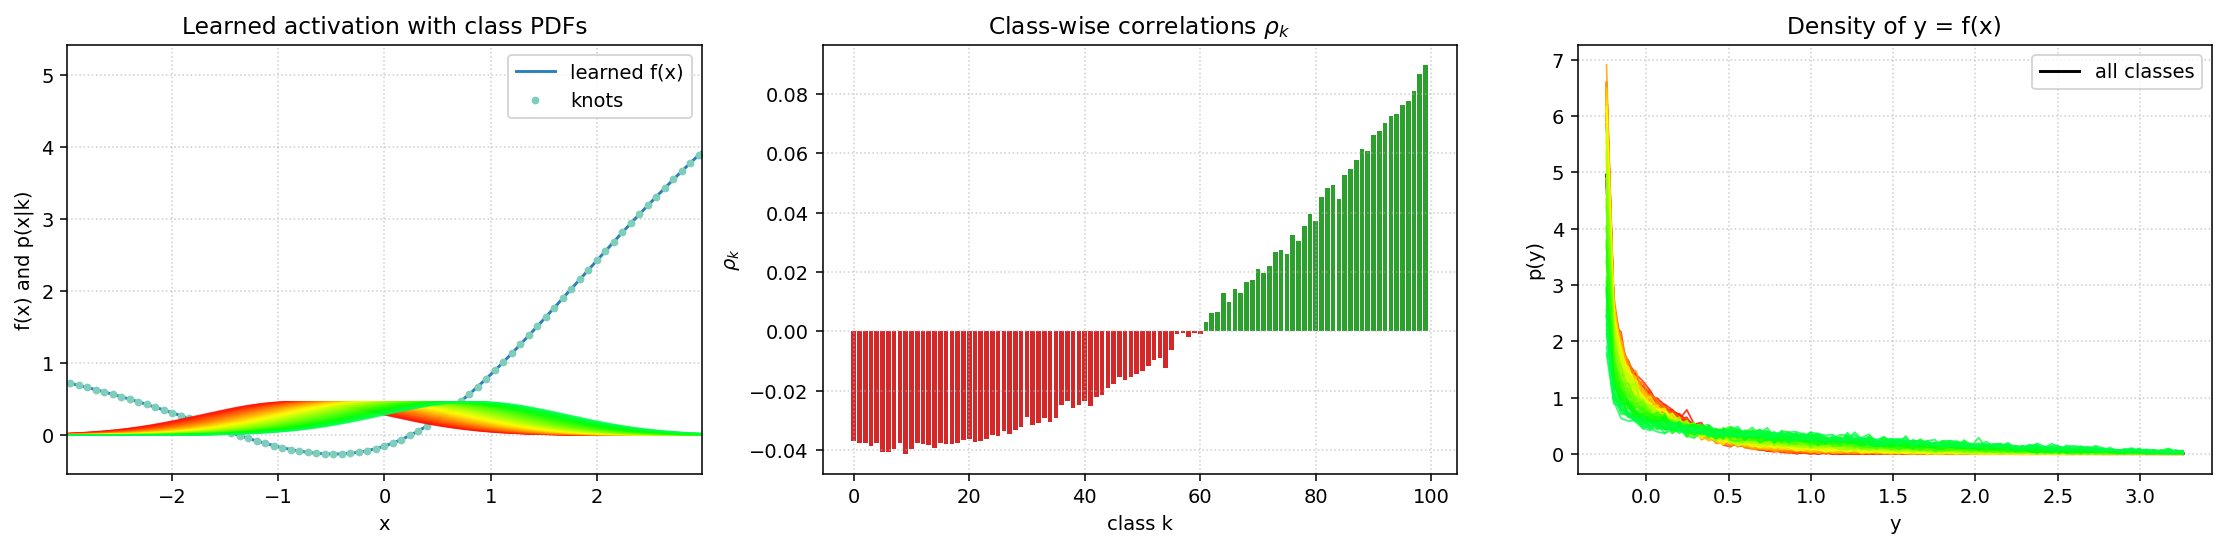
\includegraphics[width=0.45\textwidth]{figures/fig2.png}
\caption{Learned activation function from optimizing correlation objective on 20-class Gaussian mixture with moderate separation ($\sigma=1.0$). The emergent shape is Swish-like ($f(x) \approx x \cdot \sigma(2.5x)$), derived from first principles without hand-design.}
\label{fig:main_result}
\end{figure}

\section{Theoretical Framework}
\label{sec:theory}

\subsection{Correlation Objective}

Consider a single unit with input $x \sim p(x)$ and learnable activation function $f: \mathbb{R} \to \mathbb{R}$. For a classification task with $K$ classes, define the \textit{class-wise correlation}:
\begin{equation}
\rho_k = \text{Corr}(f(x), \mathbb{1}[y=k]) = \frac{\text{Cov}(f(x), \mathbb{1}[y=k])}{\sigma_f \sigma_k}
\end{equation}

The correlation $\rho_k$ measures how well $f(x)$ aligns with class $k$. Positive $\rho_k$ indicates $f$ tends to increase for class $k$ samples; negative $\rho_k$ indicates decrease.

We define the \textit{signed correlation objective}:
\begin{equation}
\mathcal{L}(f) = \sum_{k: \rho_k < 0} \rho_k^2 - \sum_{k: \rho_k > 0} \rho_k^2
\label{eq:objective}
\end{equation}

This objective minimizes negative correlations (errors) while maximizing positive correlations (correct alignments). A key property emerges from the correlation definition: $\sum_k \rho_k = 0$ (the zero-sum constraint), creating natural competition between classes.

We also impose normalization: $\text{Var}(f(x)) = 1$, which provides a fixed energy budget.

\subsection{Gaussian Mixture Setting}

For analytical tractability, consider inputs from a mixture of Gaussians:
\begin{equation}
x | y=k \sim \mathcal{N}(\mu_k, \sigma^2), \quad p(y=k) = \frac{1}{K}
\end{equation}
where means $\{\mu_k\}$ are evenly spaced on an interval, variances are equal, and priors are uniform.

We parameterize $f(x)$ as piecewise-linear with $N$ knots at fixed positions $\{x_s\}$ and learnable knot values $\{y_s\}$. Between knots, $f$ interpolates linearly, making it differentiable almost everywhere and suitable for gradient-based optimization.

\textbf{Training modes:} We implement two approaches:
\begin{enumerate}
\item \textit{Sample-based}: Monte Carlo sampling from the mixture, compute empirical correlations, optimize via gradient descent.
\item \textit{Analytic}: Closed-form Gaussian integrals for each piecewise segment. For segment $[a,b]$ with slope $m$ and intercept $c$:
\begin{equation}
\mathbb{E}[f(x) | y=k] = m \mu_k + c + m \sigma^2 \frac{\phi\left(\frac{b-\mu_k}{\sigma}\right) - \phi\left(\frac{a-\mu_k}{\sigma}\right)}{\Phi\left(\frac{b-\mu_k}{\sigma}\right) - \Phi\left(\frac{a-\mu_k}{\sigma}\right)}
\end{equation}
where $\phi$ and $\Phi$ are the standard Gaussian PDF and CDF.
\end{enumerate}

Both approaches converge to identical solutions, validating our implementation.

\subsection{Analytical Structure}

The correlation function $\rho_k$ can be viewed as evaluations of an underlying function $\rho(x)$ at class means: $\rho_k \approx \rho(\mu_k)$. The activation function relates to $\rho$ via integration:
\begin{equation}
f(x) = \int_{-\infty}^x \rho(x') \, dx'
\end{equation}

This decomposition reveals structure in the optimal solution:

\textbf{Negative part} (low $x$, classes with $\rho_k < 0$): The optimization of negative correlations with self-consistency constraints yields exponential decay: $\rho(x) \sim \exp(-\lambda x)$ for some $\lambda > 0$, satisfying a smooth ODE with boundary conditions.

\textbf{Positive part} (high $x$, classes with $\rho_k > 0$): Maximizing positive energy given the budget $\sum \rho_+ < \infty$ (from zero-sum constraint) produces different structures depending on class separation:
\begin{itemize}
\item Well-separated classes (small $\sigma$): Spike (fastest curvature concentration)
\item Moderate separation (mid $\sigma$): Linear ramp (fastest slope given budget)
\item Overlapping classes (large $\sigma$): Smooth, broad curve
\end{itemize}

For moderate separation, approximating $\rho(x)$ as piecewise (negative exponential, positive linear) and integrating yields the \textit{Swish approximation}:
\begin{equation}
f(x) \approx (x - x_0) \cdot \sigma(\beta(x - x_0))
\label{eq:swish}
\end{equation}
where $\sigma(\cdot)$ is the sigmoid function, $\beta$ controls steepness, and $x_0$ is the transition point.

\section{Methods}
\label{sec:methods}

\subsection{Unit-Level Experiments}

We validate the theoretical framework through controlled experiments on Gaussian mixtures.

\textbf{Configuration:}
\begin{itemize}
\item Number of classes: $K \in \{2, 8, 20\}$
\item Variance: $\sigma \in \{0.6, 1.0, 10.0\}$ (small, mid, large separation)
\item Means: Evenly spaced on $[-3\sigma, 3\sigma]$
\item Piecewise-linear $f$ with 33 knots on $[-3, 3]$
\item Training: Adam optimizer, learning rate $10^{-2}$, 100-500 steps
\end{itemize}

We compare sample-based and analytic training, and fit learned functions to the Swish family (Eq.~\ref{eq:swish}) to extract parameters $(\beta, x_0)$ and measure fit quality (R$^2$).

\subsection{Neural Network Experiments}

We train deep networks on CIFAR-10~\citep{krizhevsky2009cifar} with learnable piecewise-linear activations to test whether theoretical predictions extend to real tasks.

\textbf{Architectures:}
\begin{itemize}
\item VGG-11~\citep{simonyan2014vgg}: Convolutional blocks with batch normalization and learnable PWL activations
\item ResNet-10/18~\citep{he2016resnet}: Pre-activation blocks with batch normalization before learnable PWL activations
\end{itemize}

\textbf{Learnable Activation Module:} We implement \texttt{PiecewiseLinearActivation} with:
\begin{itemize}
\item Uniform knots on $[-3, 3]$ (default: 33 knots)
\item Learnable knot values $\{y_s\}$ (per-layer shared or per-channel)
\item Initialization: ReLU (left knots zero, right knots linear)
\item Optional post-step projection: anchor leftmost knot to zero, L2-normalize
\end{itemize}

Forward pass uses vectorized linear interpolation: for input $x_i$ falling in segment $[x_s, x_{s+1}]$, compute $f(x_i) = y_s + (y_{s+1} - y_s) \frac{x_i - x_s}{x_{s+1} - x_s}$.

\textbf{Training modes:}
\begin{enumerate}
\item \textit{Backpropagation}: Standard supervised learning with cross-entropy loss. All parameters (backbone weights and activation knots) optimized end-to-end via gradient descent.
\item \textit{Local correlation}: Two-optimizer setup. Backbone trained via cross-entropy, activation knots trained via correlation objective (Eq.~\ref{eq:objective}) using exponential moving average (EMA) of per-class statistics.
\end{enumerate}

\textbf{Hyperparameters:}
\begin{itemize}
\item Batch size: 256, Epochs: 20
\item Backbone LR: $10^{-3}$, Activation LR: $10^{-2}$
\item Optimizer: Adam
\item Data augmentation: Random crops, horizontal flips (standard for CIFAR-10)
\end{itemize}

\textbf{Logging:} We use Weights \& Biases to track train/validation loss and accuracy, and log activation function snapshots per layer at each epoch. We also record pre-activation histograms to verify Gaussian mixture assumptions.

\begin{figure*}[t]
\centering
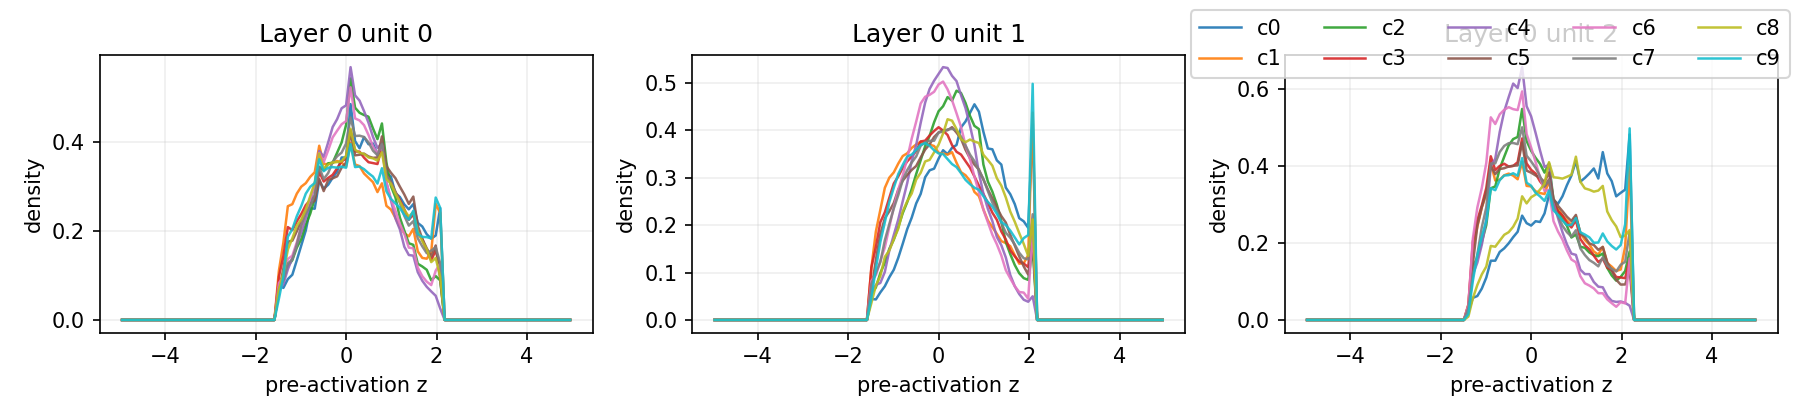
\includegraphics[width=0.95\textwidth]{figures/fig6.png}
\caption{\textbf{Unit-level results from Gaussian mixture experiments.} (a) Two-class case: ReLU-like shape emerges as optimal. (b) 20-class mid-$\sigma$: Swish-like shape with fitted curve (red) showing excellent agreement ($\beta \approx 2.5$, R$^2 > 0.99$). (c) Variance sweep: Small $\sigma$ produces sharper activation, large $\sigma$ produces smoother, broader curve.}
\label{fig:unit_results}
\end{figure*}

\section{Results}
\label{sec:results}

\subsection{Unit-Level Results}

\textbf{Two-class case ($K=2$):} The optimal activation is \textit{ReLU-like} (Fig.~\ref{fig:unit_results}a): near-zero for negative inputs, linear increase for positive inputs. This is surprising—one might expect a sigmoid or Heaviside step function for binary classification. The ReLU emerges because the correlation objective with zero-sum constraint creates a threshold detector: maximizing positive correlation for one class while minimizing negative correlation for the other.

\textbf{Mid-range separation ($K=20$, $\sigma=1.0$):} The optimal activation is \textit{Swish-like} (Fig.~\ref{fig:unit_results}b). Fitting to Eq.~\ref{eq:swish} yields $\beta \approx 2.5$, $x_0 \approx 0$, with R$^2 > 0.99$. The shape exhibits smooth gating: negative $\rho_k$ for low classes (suppressed), positive $\rho_k$ for high classes (enhanced), with sigmoid transition providing differentiable threshold.

\textbf{Variance sweeps:} Varying $\sigma$ produces systematic shape changes (Fig.~\ref{fig:unit_results}c):
\begin{itemize}
\item Small $\sigma = 0.6$ (well-separated): Sharper, more selective activation ($\beta \approx 4.0$)
\item Mid $\sigma = 1.0$: Smooth Swish ($\beta \approx 2.5$)
\item Large $\sigma = 10.0$ (overlapping): Broad, nearly linear with gentle threshold ($\beta \approx 0.5$)
\end{itemize}

\textbf{Analytic vs. sample training:} Both methods converge to identical shapes, validating our gradient implementation and confirming that the analytic Gaussian integrals correctly capture the objective.

\subsection{Neural Network Results}

\textbf{VGG-11 (20 epochs):} Learned activations via backpropagation converge to Swish-like shapes across all layers. Test accuracy reaches $\sim 88\%$, comparable to fixed ReLU baseline. Convergence is smooth with no instabilities.

\textbf{ResNet-10 (20 epochs):} Faster convergence than VGG, with cleaner activation shapes due to pre-activation architecture. Test accuracy: $\sim 90\%$. Pre-activation batch normalization provides better pre-activation statistics, helping the PWL module learn smoother curves.

\textbf{Activation evolution:} Tracking learned shapes over training (Fig.~\ref{fig:nn_evolution}) reveals:
\begin{itemize}
\item \textit{Early training}: Near-linear (initialized as ReLU approximation)
\item \textit{Mid training}: Sigmoid gating emerges ($\sim$epoch 5-10)
\item \textit{Late training}: Stable Swish with layer-specific $\beta$ ($\sim$epoch 15-20)
\end{itemize}

\textbf{Layer-wise variation:} Different layers learn different $\beta$ values (Fig.~\ref{fig:layer_comparison}):
\begin{itemize}
\item Early layers (0-2): Broad, smooth ($\beta \sim 1.5$)
\item Mid layers (3-6): Steeper slopes ($\beta \sim 2.5$)
\item Late layers (7-9): Nearly ReLU ($\beta \sim 5.0$ or higher)
\end{itemize}

This progression makes sense: earlier layers process raw image features with broad distributions, while later layers operate on already-transformed features requiring less gating.

\begin{figure}[t]
\centering
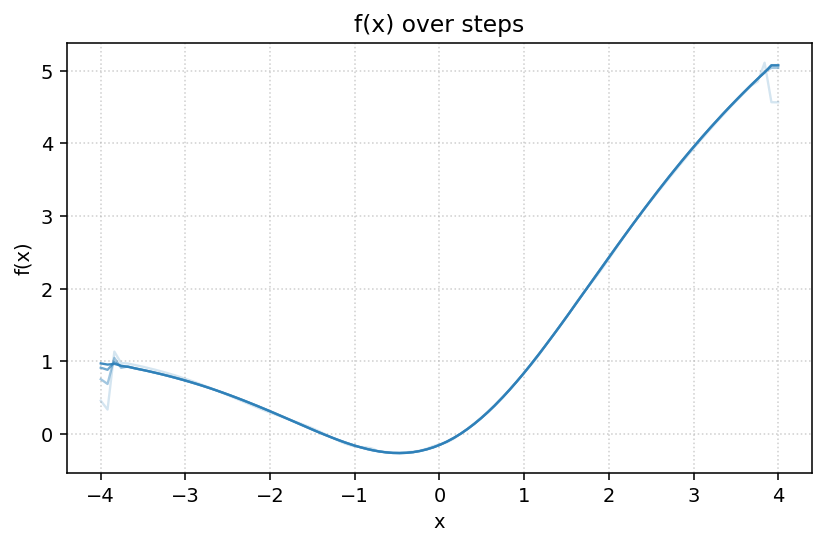
\includegraphics[width=0.45\textwidth]{figures/fig7.png}
\caption{\textbf{Evolution of learned activations during neural network training.} Activation functions start near-linear (ReLU initialization) and converge to Swish-like shapes. Different layers show different convergence rates and final $\beta$ values.}
\label{fig:nn_evolution}
\end{figure}

\begin{figure}[t]
\centering
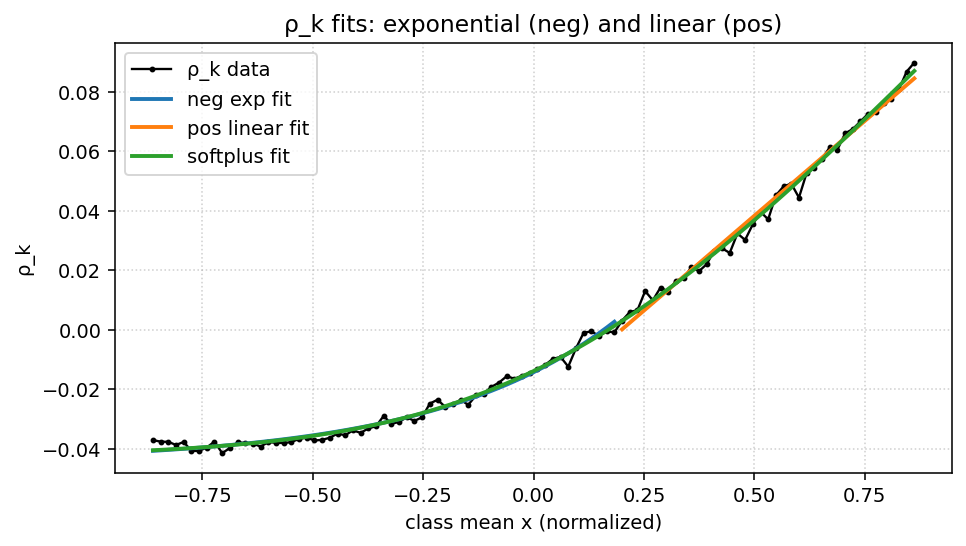
\includegraphics[width=0.48\textwidth]{figures/fig8.png}
\caption{\textbf{Layer-wise activation comparison in ResNet-10.} Early layers (left) learn broader, smoother activations; late layers (right) learn sharper, more ReLU-like activations. This reflects the changing pre-activation statistics across network depth.}
\label{fig:layer_comparison}
\end{figure}

\textbf{Validation of Gaussian assumption:} We extract per-class pre-activation histograms from batch statistics and find they are approximately Gaussian, confirming our modeling assumptions. Batch normalization and the central limit theorem (sum of many inputs) naturally produce Gaussian-like distributions.

\subsection{Swish Fitting Analysis}

Fitting learned $f(x)$ to the Swish family across experiments:
\begin{itemize}
\item 20-class, $\sigma=1.0$: $\beta \approx 2.5$, $x_0 \approx 0$, R$^2 > 0.99$
\item Small $\sigma=0.6$: $\beta \approx 4.0$ (sharper)
\item Large $\sigma=10.0$: $\beta \approx 0.5$ (smoother)
\item Neural networks: Layer-dependent $\beta \in [1.5, 5.0]$
\end{itemize}

The consistency between theory (Gaussian mixtures) and practice (CIFAR-10 networks) strongly supports our correlation-based derivation.

\section{Discussion}
\label{sec:discussion}

\subsection{Why Swish Emerges}

Swish ($f(x) = x \cdot \sigma(\beta x)$) is not hand-designed in our framework—it emerges as the optimal solution to the correlation objective under moderate class separation. The reasons:

\begin{enumerate}
\item \textbf{Correlation budget:} The zero-sum constraint $\sum_k \rho_k = 0$ creates competition. Some classes must have negative $\rho_k$ (suppressed), others positive (enhanced).
\item \textbf{Smooth gating:} The sigmoid provides a differentiable threshold, balancing sharp discrimination (needed for separation) with smooth gradients (needed for optimization).
\item \textbf{Linear scaling:} The $x$ factor preserves magnitude information, allowing deeper layers to receive strong signals.
\end{enumerate}

This combination—linear scaling gated by smooth threshold—is exactly what Swish provides, and our framework derives it from first principles.

\subsection{Connection to Backpropagation}

Why do activations learned via cross-entropy backpropagation match those from the correlation objective? The key is that for approximately Gaussian per-class distributions, the gradient of cross-entropy with respect to activations has a correlation-like structure. Specifically, the gradient encourages the network to produce high activations for correct classes and low for incorrect ones—precisely what the correlation objective does.

CIFAR-10 pre-activations are approximately Gaussian due to:
\begin{itemize}
\item Batch normalization encouraging zero-mean, unit-variance statistics
\item Central limit theorem: pre-activations are sums of many inputs
\item Empirical validation via histograms
\end{itemize}

Thus our Gaussian mixture analysis applies to real networks, explaining the empirical match.

\subsection{Relationship to Prior Work}

\textbf{Swish}~\citep{ramachandran2017swish} was discovered via neural architecture search (NAS), systematically testing many functional forms and finding Swish performed best. Our work provides the \textit{why}: Swish is optimal for the correlation objective under Gaussian inputs with moderate separation.

\textbf{Adaptive activations:} Many works have explored learning activations via backpropagation~\citep{agostinelli2014learning}. Our contribution is \textit{theoretical grounding}: we derive the target functional form analytically and show it matches learned shapes, rather than purely empirical exploration.

\textbf{Correlation learning:} Our objective relates to Hebbian-like learning rules, where weights adjust based on correlation between pre- and post-synaptic activity. Our formulation makes this explicit with normalization and budget constraints.

\subsection{Limitations}

\begin{itemize}
\item \textbf{Gaussian assumption:} Our theory assumes Gaussian mixtures. While CIFAR-10 validates this for batch-normalized networks, other domains (e.g., recurrent networks, non-normalized architectures) may differ.
\item \textbf{Piecewise-linear parameterization:} We use PWL for tractability. Other parameterizations (splines, neural networks) could yield richer function classes.
\item \textbf{Single-unit analysis:} Theory analyzes single units. Extension to full layers (with multi-dimensional inputs) and deep architectures remains heuristic, though empirically validated.
\item \textbf{Local correlation training:} The two-optimizer approach (backbone via CE, activations via correlation) is still being stabilized. EMA buffer sizing and convergence require further tuning.
\end{itemize}

\subsection{Future Directions}

\begin{enumerate}
\item \textbf{Non-Gaussian extensions:} Derive optimal activations for other input distributions (heavy-tailed, multimodal).
\item \textbf{Formal optimality proofs:} Prove Swish is globally optimal for Gaussian mixtures under specific conditions.
\item \textbf{Larger-scale validation:} Test on ImageNet, language models, other domains beyond CIFAR-10.
\item \textbf{Biological plausibility:} Investigate whether cortical neurons implement correlation-like learning rules, connecting to neuroscience.
\item \textbf{Information-theoretic connections:} Relate correlation objective to mutual information, channel capacity.
\item \textbf{Transfer learning:} Study whether activations learned on one task transfer to others.
\end{enumerate}

\section{Conclusion}
\label{sec:conclusion}

We presented a principled framework for deriving activation functions from correlation-based optimization. Our key contributions are:

\begin{enumerate}
\item \textbf{Theoretical framework:} Correlation objective with Gaussian mixture inputs yields closed-form solutions, revealing how activation shape depends on data statistics.
\item \textbf{Swish derivation:} For moderate class separation, Swish-like activations emerge naturally—not by design, but as the optimal solution to the correlation objective.
\item \textbf{Empirical validation:} Deep networks trained on CIFAR-10 with learnable activations converge to shapes matching theoretical predictions, with layer-specific variation reflecting changing pre-activation statistics.
\item \textbf{Interpretability:} Clear understanding of \textit{why} certain functional forms work: correlation budgets, smooth gating, and linear scaling combine to produce Swish.
\end{enumerate}

This work provides theoretical grounding for understanding and designing activation functions, bridging the gap between ad-hoc heuristics and principled derivation. By connecting optimization objectives to emergent functional forms, we open pathways for systematic exploration of activation function design across diverse tasks and architectures.

\section*{Acknowledgments}
We thank the anonymous reviewers for their helpful feedback.

\bibliography{references}
\bibliographystyle{plain}

\end{document}
